\documentclass[12pt]{article}
\usepackage{tikz}
\usepackage{pgfplots}
\pgfplotsset{compat=1.13}

\usepackage{extsizes}
\usepackage{caption}
\usepackage{multirow}
\usepackage{wrapfig}

\renewcommand{\epsilon}{\ensuremath{\varepsilon}}
\renewcommand{\phi}{\ensuremath{\varphi}}
\renewcommand{\kappa}{\ensuremath{\varkappa}}
\renewcommand{\le}{\ensuremath{\leqslant}}
\renewcommand{\leq}{\ensuremath{\leqslant}}
\renewcommand{\ge}{\ensuremath{\geqslant}}
\renewcommand{\geq}{\ensuremath{\geqslant}}
\renewcommand{\emptyset}{\varnothing}

\newcommand{\lw}{\linewidth}
\usepackage{geometry} % Простой способ задавать поля
\geometry{top=30mm}
\geometry{bottom=30mm}
\geometry{left=25mm}
\geometry{right=20mm}

\usepackage[T2A]{fontenc}			% кодировка
\usepackage[utf8]{inputenc}	
\usepackage[english,russian]{babel}   %% загружает пакет многоязыковой вёрстки
\usepackage{indentfirst}
\usepackage{subfigure}
\usepackage{amsmath,amsfonts,amssymb,amsthm,mathtools} 
\usepackage{graphicx}

\usepackage{pdfpages}

\begin{document}
	\begin{minipage}{0.45\linewidth}
	Работу выполнили\\
	Самохин Валентин,\\
	Юрченко Петр\\ 676 гр.\\[2mm]
	под руководством\\
	Нухова А.\,К\,.
	\end{minipage}
	\hfill
	\begin{minipage}{0.45\linewidth}\flushright
		Маршрут~VIII \ №~6\\[3mm]
		10~апреля 2018~г.,\\
		\end{minipage}
		
		\vspace{8mm}
		\begin{center}
			\textbf{\Large Лабораторная работа №~4.3.2:}\\[\parskip]
			\LARGE Изучение дифракции света
			\end{center}
			\vspace{0mm}
			\paragraph{Цель работы:}
	изучение дифракции света на синусоидальной акустической решетке и наблюдение фазовой решетки методом темного поля.
				

			
			\paragraph{В работе используются:}
			оптическая скамья, осветитель, два длиннофокусных объектива, кювета с жидкостью, кварцевый излучатель с микрометрическим винтом, генератор ультразвуковой частоты, линза, вертикальная нить на рейтере, микроскоп.
			
			
			
			\vspace{2\parskip}
		\paragraph{Теоретическая справка.}
		 В работе изучается дифракция света на фазовой решетке, которая создается в жидкости ультразвукрвыми волнами --- возникают периодические оптические неоднородности. Если считать акустическую решетку неподвижной, а вызванное ультразвуком возмущение показателя преломления малым, то эту решетку можно рассматривать как тонкий фазовый экран. 
		 
		 При небольших амплитудах звуковой волны показатель преломления жидкости $n$ меняется по закону $$n = n_0(1+m\cos\Omega x),$$
		 где $\Omega$ - волновое число для УЗ-волны.
		 
		 Пусть фаза световых колебаний на передней поверхности жидкости равна нулю. Тогда на задней поверхности (т.е. в плоскости $z = 0$) она равна 
		 $$\phi = knL = \phi_0(1 + m\cos \Omega x),$$
		 где $L$ - толщина слоя жидкости в кювете, $k$ - волновое число для света, $\lambda$ - длина световой волны, $$\phi_0 = kn_0L.$$ Таким образом, УЗ-волна в жидкости создает фазовую дифракционную решетку.
		 
		 Условие, при выполнении которого можно считать акустическую решетку тонким фазовым экраном, можно записать в виде $$m \ll \dfrac{\Lambda}{L}\sqrt{\dfrac{\lambda}{L}}.$$
		 
		 \subparagraph{Дифракция Френеля на амплитудной синусоидальной решетке.}
		 Функция пропускания решетки с периодом $d = \dfrac{2\pi}{\Omega}$:
		 $$t(x) = 1 + m\cos\Omega x \;(m < 1).$$
		 Разложив косинус, находим 
		$$f_0(x) = a + \dfrac{am}{2}e^{i\Omega x} + \dfrac{am}{2}e^{-i\Omega x}.$$
		
		Комплексная амплитуда волны в плоскости $z$, удовлетворяющая граничному условию, имеет вид 
		$$f(x,z) = ae^{ikz} + \dfrac{am}{2}e^{i(\Omega x + \sqrt{k^2 - \Omega^2}z)} + \dfrac{am}{2}e^{i(-\Omega x + \sqrt{k^2 - \Omega^2}z)} .$$
		
		Полагаем, что период решетки существенно больше длины волны $\lambda$ и, следовательно частоты решетки много меньше $k$: $\Omega \ll k$. Тогда преобразований получаем 
		$$f(x,z) = ae^{ikz}\left[1 + me^{-i\frac{z}{2k}}\right]$$
		
		Из этой формулы можно показать, что видность наблюдаемой дифракционной картины изменяется периодически по $z$. Причина этих изменений - в различии фазовых набегов трех плоских волн.
		
		\subparagraph{Дифракция на фазовой синусоидальной решетке. }
		
		В данном случае функция пропускания: $$t(x) = e^{im\cos \Omega x}$$
		Полагая $m \ll 1$, получаем $$t(x) \approx 1 + \dfrac{im}{2}e^{i\Omega x} + \dfrac{im}{2}e^{-i\Omega x}$$
		При освещении этой решеткой плоской нормально падающей волной амплитуды $a$ за решеткой имеем: $$f(x,z) = ae^{ikz} + \dfrac{iam}{2}e^{i(\Omega x + \sqrt{k^2 - \Omega ^2}z)} + \dfrac{iam}{2}e^{i(-\Omega x + \sqrt{k^2 - \Omega ^2}z)}$$
		Сравнивая результат с предыдущим случаем, видим что три волны имеют те же амплитуды и направления распространения, оличие лишь в начальных фазах.
		
		\subparagraph{Метод темного поля.}
		Важным понятием является фурье-плоскость. Если при рассматривании формирования изображения с помощью линзы основываясь на идее пространственного спектральног разложения. Каждая гармоника --- плоская волна определенного направления --- фокусируется линзой в отдельную точку фокальной плоскости. 
		 По этой причине фокальную плоскость линзы называют \textit{фурье-плоскостью}. Далее каждая точка фурье-плоскости рассматривается как источник сферической волны.
		
		 Устанавливая в фурье-плоскости различные амплитудно-фазовые маски, можно направленно изменять пространственный спектр изображения, влияя таким образом на его характеристики.
		 
		 Пусть фазовый объект - тонкая прозрачная пластика, имеющая разный в разных точках показатель преломления, но не изменяющая амплитуду прошедней волны. Функция пропускания такой пластинки есть $t(x) = e^{i\phi(x)}$, где $\phi(x) = kn(x)d$.
		 
		 Для визуализации фазового объекта Цернике предложил установить в фурье-плоскости, на оптической оси, маленькую фильтрующую пластинку, которая, не изменяя амплитуды прошедшей волны, вносит фазовую задержку, равную $\pi/2$.  
		 \begin{center}
		 	
		 
		 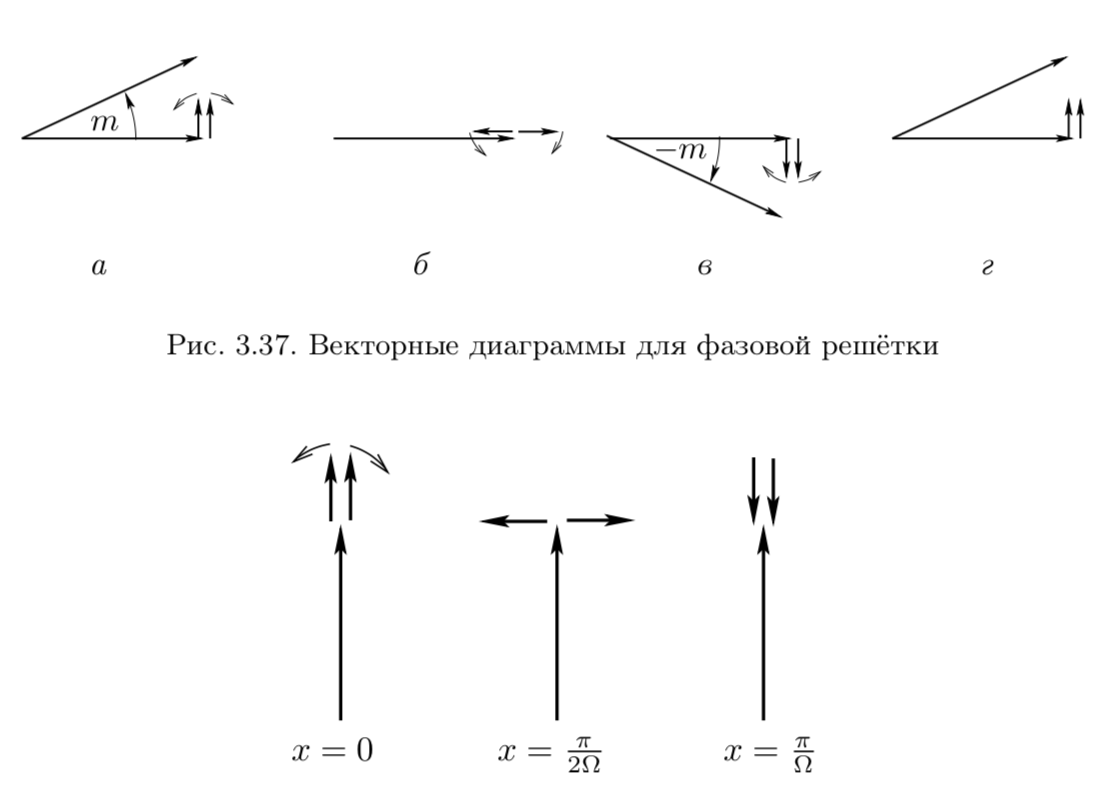
\includegraphics[scale=.8]{faz_diags}
		\end{center}
		 Пусть объект - фазовая синусоидальная решетка с малой глубиной модуляции. В этом случае 
		 $$f_0(x) = e^{im\cos \Omega x} \approx 1 +  \dfrac{im}{2}e^{i\Omega x} + \dfrac{im}{2}e^{-i\Omega x}$$
		 
		 Осевая плоская волна, фокусируясь линзой в начало координат фурье плоскости, проходит через фазовую фильтрующую пластинку, а две наклонные волны, фокусируясь в точки $\pm f\frac{\Omega}{k}$, не задевают пластинку. Далее линза преобразует сферические волны, исходящие из этих трех точек на фурье-плоскости, в плоские волны, которые интерферируя, образуют изображение.
		 
		 Таким образом, метод фазового контраста позволяет преобразовать исходную фазовую решетку в амплитудную решетку в плоскости изображения.
		 
		 Наблюдаемая картина интенсивности имеет вид
		 $$I(x)  = |f(x)|^2 \approx (1 + m\cos\Omega x)^2 \approx 1 + 2m\cos\Omega x$$
		 
		  Итак, фазовые изменения оказались визуализированы изменениями интенсивности, повторящими изменения фазы входного поля.
		  
		  В \textit{методе темного поля} вместо фазовой пластинки в фурье-плоскости на оптической оси устанавливается непрозрачный маленький экран. Поле в выходной плоскости в этом случае имеет вид
		  $$f(x) = im\cos\Omega x,$$
		  а интенсивность - $$I(x) = m^2\cos^2\Omega x.$$
		  
		  \subparagraph{Опыт.}
		  Вернемся к нашему опыту с кюветой.
		  Определяя на опыте положение дифракционных максимумов различного порядка, можно по формуле $\Lambda\sin\theta_m = m\lambda$ найти длину УЗ-волны и вычислить скорость распространения УЗ-волн в жидкости, если известна частота колебаний кварцевого излучателя.
		  
		  \paragraph{Экспериментальная установка.}
		   \subparagraph{Наблюдение дифракции}
		  Для наблюдения дифракции света на УЗ-волнах на оптической скамье собирается следующая установка.
		  \begin{center}
		  	
		 
	  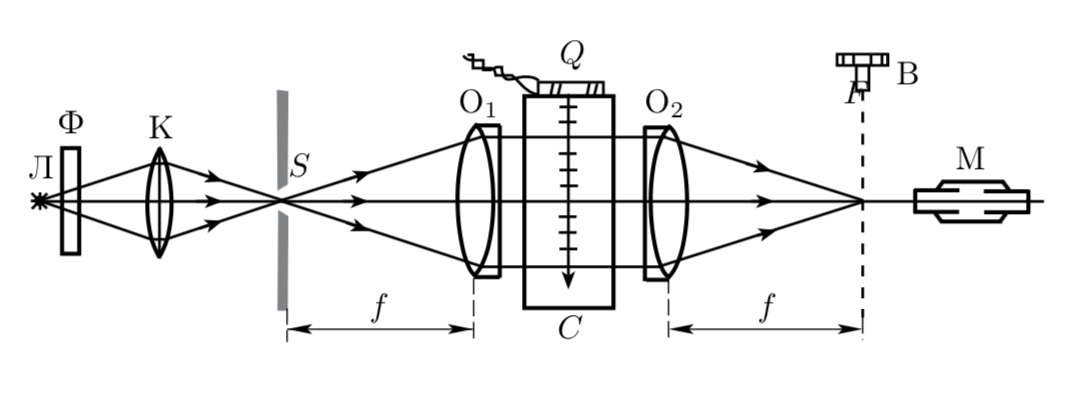
\includegraphics[scale=.7]{first}
\end{center}
		В фокальной плоскости второго объектива образуется дифракционная картина, наблюдаемая при помощи микроскопа. 
		
		Длина УЗ-волны определяется с помощью $$\Lambda\sin\theta_m = m\lambda$$ и в силу малости углов это выражение может быть представлено в виде 
		\begin{equation}\label{eq::for_uz_len}
		l_m = mf\dfrac{\lambda}{\Lambda}
		\end{equation}
		
		где $l_m$ - измеренное на опыте линейное расстояние между $m$ - м и нулевым максимумами, а $f$ - фокусное расстояние второго объектива.
		
		\subparagraph{Наблюдение акустической решетки методом темного поля.}
		
		Прежде всего в поле зрения микроскопа получают изображение задней плоскости кюветы. Затем используя метод темного поля, с помощью специального экрана устраняется центральный дифракционный максимум. Нетрудно показать, что в поле зрения микроскопа будут наблюдаться чередующиеся светлые и темные полосы, причем расстояние между темными полосами соответствует смещению в плоскости кюветы на $\Lambda / 2$. Таким образом, должно наблюдаться характерное для метода темного поля удвоение числа деталей рассматриваемой структуры. 
		\begin{center}
		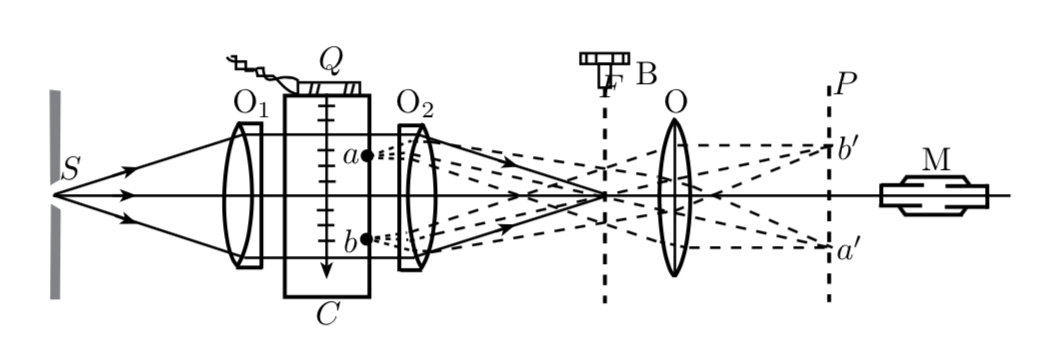
\includegraphics[scale=.7]{second}
		\end{center}
		Отметим, что этот опыт можно проводить только со стоячими волнами, т.к. в случае бегущей волны визуальное наблюдение оказывается невозможным.
		
		\subparagraph{Установка с горизонтальной щелью.}
		.
		
		\begin{center}
		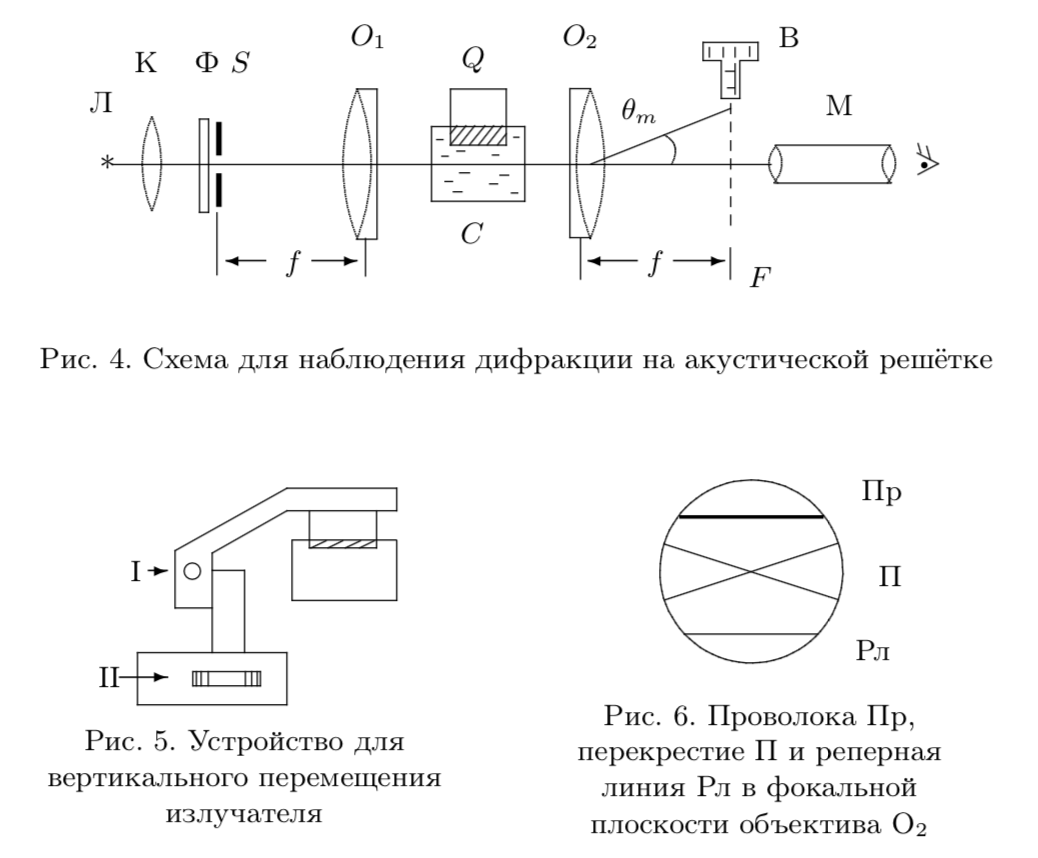
\includegraphics[scale=.6]{horizontal}
		\end{center}
	
	\paragraph{Выполнение работы.}
	В работе предлагается измерить координаты полос, образующихся при дифракции света на акустической решетке, а также определить период этой решетки методом темного поля. По результатам измерений рассчитывается скорость ультразвука в воде. Все измерения ведутся на стоячей волне.
	
	\subparagraph{Определение скорости ультразвука по дифракционной картине.}
	Предварительно проведя тщательную настройку установку, получим дифракционную картину. К сожалению, больше семи полос получить не удалось ни в одном опыте. Тем не менее, для трех частот генератора мы сняли зависимость координаты $Y$ в делениях винта от номера полосы $m$ для каждой светлой полосы. Из \eqref{eq::for_uz_len}, зная коэффициент наклона прямой, выражающей зависимость $Y(m)$, нетрудно выразить длину УЗ-волны, а затем рассчитать скорость звука для каждой частоты.
	
	\begin{center}
		
		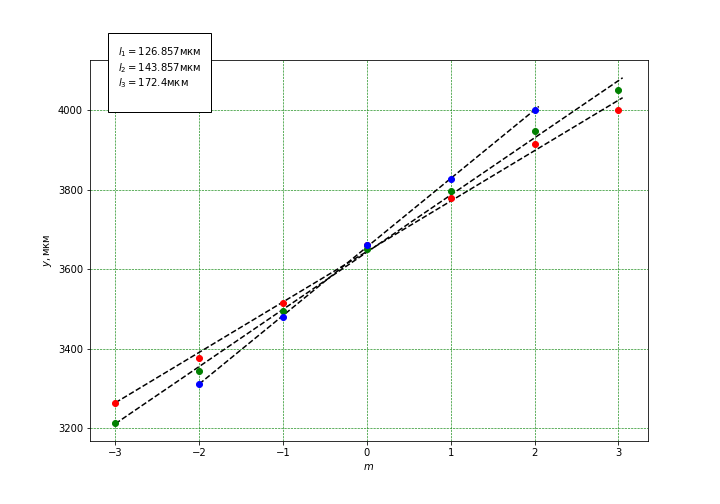
\includegraphics[scale=.6]{speed_by_difr}
		\captionof{figure}{Зависимость $Y(m)$ для трех различных частот генератора}
	\begin{tabular}{|c|c||c|c||c|c|}
		\hline 
		\multicolumn{2}{|c||}{$\nu_1 = 1,09 MHz$} &  	\multicolumn{2}{|c||}{$\nu_2= 1,2 MHz$}  & 	\multicolumn{2}{|c|}{$\nu_3 = 1,4 MHz$} \\ 
		\hline 
		\hline
		$m$ & $Y$, дел. винта  & $m$ & $Y$, дел. винта  & $m$ & $Y$, дел. винта  \\
		\hline
		$-3$& $8,16$ & $-3$ & $8,03$  & $-3$ & - \\ 
		\hline 
		$-2$& $8,44$ & $-2$ & $8,36$ & $-2$ & $8.28$ \\ 
		\hline 
		$-1$ & $8,79$ & $-1$ & $8,74$ & $-1$ & $8,7$  \\ 
		\hline 
		$0$& $9,15$ & $0$ & $9,13$ & $0$ & $9,15$ \\ 
		\hline 
		$1$& $9,45$ & $1$ & $9,49$ & $1$ & $9,57$  \\ 
		\hline 
		$2$& $9,79$ & $2$ & $9,87$ & $2$ & $10$ \\ 
		\hline 
		$3$& $10$ & $3$ & $10,13$ & $3$ & -  \\ 
		\hline 
		\hline
		\multicolumn{2}{|c||}{$\Lambda_1 = 1,41 \pm 0,04\ mm$} &  \multicolumn{2}{|c||}{$\Lambda_2 = 1,25 \pm 0,04\ mm$}  &  \multicolumn{2}{|c|}{$\Lambda_3 = 1,04 \pm 0,03\ mm$}\\ 
		\hline 
		\multicolumn{2}{|c||}{$c_1 = 1,54\ km/s$} &  \multicolumn{2}{|c||}{$c_2 = 1,49\ km/s$}  &  \multicolumn{2}{|c||}{$c_3 = 1,46\ km/s$} \\ 
		\hline
		\hline
		\multicolumn{6}{|c|}{$\overline{c} = 1,49\ m/s$}\\
		\hline 
	\end{tabular} 
	\captionof{table}{Данные для определения скорости ультразвука по дифракционной картине}
	\end{center}


При вычислениях использовались значения: фокусного расстояния $O_2$ $f = 28\ cm$, длины волны красного цвета  $0,64 \pm 0,02$ мкм, а также цены деления винта $400$ мкм
\subparagraph{Определение скорости ультразвука методом темного поля.}

Прежде всего рассчитаем цену малого деления окулярной шкалы: она равняется $4/1,64$ мм.

Далее, закрыв нулевой дифракционный максимум, пронаблюдаем акустическую решетку. Заметим, что при удалении проволоки с главного максимума решетка не видна. 

Зафиксируем с помощью окулярной шкалы микроскопа координаты первой и последней из хорошо видимых в поле зрения темных полос и количество светлых промежутков между ними для нескольких частот УЗ-излучателя.

Наконец, для каждой частоты определим длины УЗ-волны с учетом удвоения числа наблюдаемых полос. Построив график $\Lambda = F(1/\nu)$, по наклону прямой найдем скорость ультразвука в воде.

\begin{center}
	
\begin{tabular}{|c|c|c|c|c|}
	\hline 
	$\nu, MHz$ & $x_l$, дел. шкалы & $x_r$, дел. шкалы & $m$ & $\Lambda$, мм \\ 
	\hline 
	\hline
	$1$& $1,38$  & $3,22$  & $6$ & $1,50 \pm 0,01$ \\
	\hline 
	$1,08$ & $1,08$ & $3,08$ & $7$ & $1,39 \pm 0,02$\\
	\hline
	$1,17$ & $0,94$ & $3,04$ & $8$ & $1,28 \pm 0,02$\\
	\hline
	$1,24$ & $0,94$ & $3,42$ & $10$ & $1,21 \pm 0,02$\\
	\hline
	$1,35$ & $0,9$ & $3,42$ & $11$ & $1,12 \pm 0,02$\\
	\hline
	$1,45$ & $1,06$ & $3,00$ & $9$ & $1,05 \pm 0,01$\\
	\hline 
\end{tabular} 
\captionof{table}{Данные для расчета скорость звука с помощью метода темного поля}

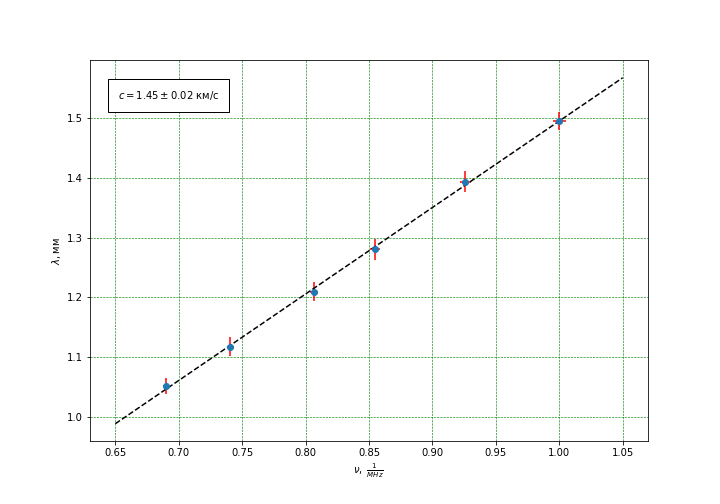
\includegraphics[scale=.6]{speed_by_dark_field}
\captionof{figure}{График зависимости $\Lambda = f(1/\nu)$}

$\boxed{c = 1,45 \pm 0,02\ km/s}$
\end{center}

\paragraph{Вывод.} 

Мы изучили дифракцию света на синусоидальной акустической решетке и пронаблюдали фазовую решетку методом темного поля. Результатом наших измерений стало значение скорости звука в воде, которое оказалось равным табличному.
\end{document}